\documentclass{standalone}
\usepackage{fontspec}
\setsansfont{DejaVuSans.ttf}[Path=./,Kerning=Off,Ligatures={TeXOff,NoCommon}]
\usepackage{tikz}
\begin{document}
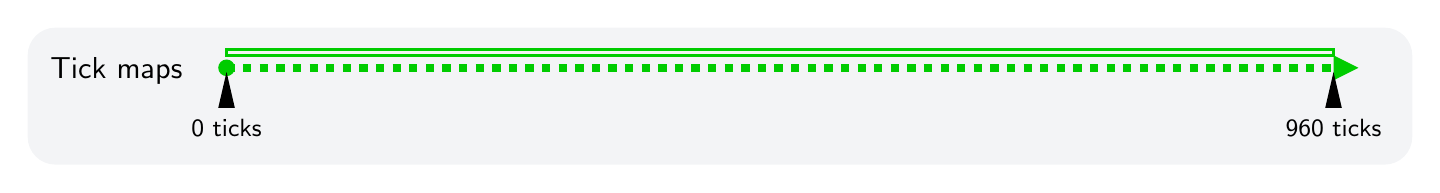
\begin{tikzpicture}[x=1pt,y=1pt,miter limit=4,font=\sffamily]
\definecolor{ts000000}{HTML}{000000}
\definecolor{ts00CC00}{HTML}{00CC00}
\definecolor{tsF3F4F6}{HTML}{F3F4F6}
\begin{scope}[shift={(16,16)}]
\path[rounded corners=10pt,fill=tsF3F4F6] (0,0) rectangle (500.3181,49.4766);
\path[draw=ts00CC00,line width=1pt] (71.8594,41.4766) -- (471.8594,41.4766) -- (471.8594,39.4766) -- (71.8594,39.4766) -- cycle;
\path[draw=ts00CC00,line width=3pt,dash pattern=on 3pt off 3pt] (71.8594,34.9766) -- (471.8594,34.9766);
\path[fill=ts00CC00] (71.8594,34.9766) circle[radius=3];
\path[fill=ts00CC00] (480.8594,34.9766) -- (471.8594,39.4766) -- (471.8594,30.4766) -- cycle;
\path[fill=ts000000] (71.8594,33.4766) -- (68.8594,20.4766) -- (74.8594,20.4766) -- cycle;
\path[fill=ts000000] (471.8594,33.4766) -- (468.8594,20.4766) -- (474.8594,20.4766) -- cycle;
\node[anchor=base west,inner sep=0,font=\sffamily\fontsize{11}{12.8047}\selectfont,text=ts000000] at (8,31.1685) {Tick maps};
\node[anchor=base,inner sep=0,font=\sffamily\fontsize{9}{10.4766}\selectfont,text=ts000000] at (71.8594,10.1226) {0 ticks};
\node[anchor=base,inner sep=0,font=\sffamily\fontsize{9}{10.4766}\selectfont,text=ts000000] at (471.8594,10.1226) {960 ticks};
\end{scope}
\end{tikzpicture}
\end{document}
